\section{Finding 5 - SSLv2, SSLv3, TLS 1.1 support}
\hrule
\begin{table}[htb]
    \renewcommand{\arraystretch}{1.5}
    \begin{tabular*}{\textwidth}{|>{\columncolor{red!15}}p{3cm}|p{17.2cm}|}
    \textbf{Finding} & \textbf{SSLv2, SSLv3,TLS 1.1 support}\\
    Risk& High\\
    Category & Misconfiguration, Patching\\
    Impact& Decrypt Data, Man in the Middle Attacks \\\\ 
    Description& The \ac{tls} configuration supports the deprecated protocols: SSLv2, SSLv3, TLS 1.1. Executing the command:\newline
    ''openssl s\_client --connect 172.16.0.29:433 -ssl2''\newline
    opens an SSLv2 connection to the server 172.16.0.29 on port 433 and displays the encryption and certificate information.
    \newline
    \newline
    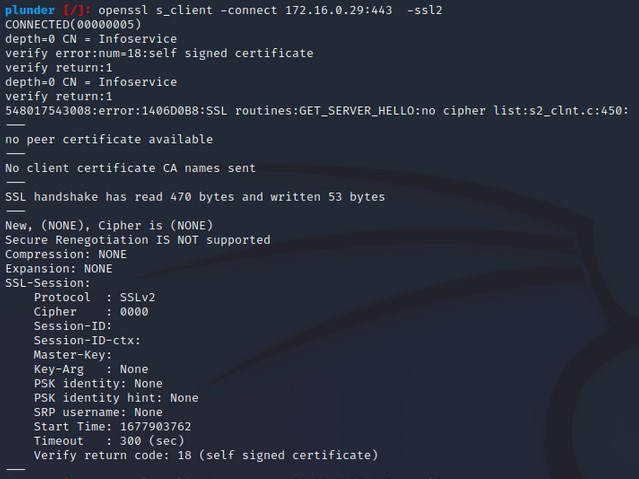
\includegraphics[width=0.73\textwidth]{ssl_2_support.jpg}
    \newline
	\\ 
    Recommendation& Change your TLS configuration and disable support for the insecure protocols: SSLv2, SSLv3, TLS 1.1\\    
    \end{tabular*}
    \end{table}